\documentclass[a4paper,10pt]{article}

\usepackage[utf8]{inputenc}
\usepackage[english]{babel}
\usepackage[T1]{fontenc}
\usepackage{mathpazo}

\usepackage[colorlinks=true]{hyperref}
\hypersetup{urlcolor=black,linkcolor=black}

\usepackage{enumerate}

\usepackage{fullpage}
\setlength{\parindent}{0pt}
\setlength{\parskip}{\medskipamount}

\usepackage{amsmath}
\usepackage{amssymb}
\usepackage{mathrsfs}
\usepackage{amsthm}
\usepackage{array}
\usepackage{graphicx}
\usepackage{comment}
\usepackage{pgfgantt}

\newcounter{wpcounter}
\newenvironment{workpackage}{\stepcounter{wpcounter}\vspace{0.5cm}{\bfseries WP\thewpcounter}}{}

\title{Midterm report}
\author{PPP \--- ENS Lyon}
\date{M1. 2014}
\begin{document}
\maketitle

\newlength{\title}
\settowidth{\title}{Coordinator }

\newlength{\object}
\setlength{\object}{\textwidth} \addtolength{\object}{-\title} \addtolength{\object}{-6.8pt} 
    \addtolength{\object}{-2\tabcolsep}

\renewcommand{\arraystretch}{1.5}

\begin{center}
\begin{tabular}{@{}|p{\title}p{\object}@{}|}
\hline
Title & Projet Pensées Profondes (PPP)\\
Coordinator & Marc \textsc{Chevalier}\\
Members & Raphaël \textsc{Charrondière}, Marc \textsc{Chevalier}, Quentin 
      \textsc{Cormier}, Tom \textsc{Cornebize}, \linebreak Yassine \textsc{Hamoudi}, 
      Valentin \textsc{Lorentz} and Thomas \textsc{Pellissier} \textsc{Tanon}.\\
Abstract & \emph{Projet Pensées Profondes} aims to build a natural language question answering framework.
It is done at the ENS Lyon, from September to December 2014, by a team of seven M1 students. This proposal presents
our subject and exposes our goals.\\
\hline
\end{tabular}
\end{center}
\tableofcontents

The {\em Projet Pensées Profondes} (Deep Thought Project) aims at
providing a powerful software for answering questions written in
natural language.
To accomplish this, we developped an eponymous set of tools that
accomplish different tasks and fit together thanks to a protocol
we developped.

These various tasks include data querying (using the young and open
knownledge base Wikidata), question parsing (using the
CoreNLP software written by Stanford University and machine learning),
requests routing, web user interface, and feedback reporting.

Given the young age of this projet, these pieces are only starting
to emerge with their first features and mutual communications,
so we will describe them separately in this document without
much of a general overview of the project.


\section{Communications}

As its name suggests, the core is the central point of the PPP. It is
connected to all other components — user interfaces and modules — through
the protocol defined above.

The core communicates with the user interfaces and the modules {\em via} HTTP:
each time the core receives a requests from an interface, it forwards it
to modules, using a configurable list of URL where to reach modules.

An example configuration is the one we use on the production server:

\begin{verbatim}
{
    "debug": false,
    "modules": [
        {
            "name": "nlp_classical",
            "url": "http://localhost:9000/nlp_classical/",
            "coefficient": 1
        },
        {
            "name": "flower",
            "url": "http://localhost:9000/flower/",
            "coefficient": 1
        },
        {
            "name": "wikidata",
            "url": "http://wikidata.ppp.pony.ovh/",
            "coefficient": 1
        }
    ]
}
\end{verbatim}

The current state is the the Core is successfully able with all modules
that have been written: the Wikidata module, an example Python module
(which answers the question  “Who are you?”), and the Natural Language
Processing module.

\section{Routing}

Besides from communicating with other pieces of the PPP, the Core will
also route requests in such a way the power of the modules can be
combined to give something greater.

For instance, when a user will input a question like “Who is the first
president of the United States?”, the Core will send the question to
all modules and get a parsed tree from the Natural Language Processing
module. Then, it will forward this answer to all other modules, which the
Wikidata module will be able to answer.

This part is not implemented, but will be next step in the implementation
of the Core.


\chapter{User Interface}

We decided to implement first only a web user interface. This interface
is only composed of one web-page developed in HTML 5 with some
pieces of JavaScript and CSS. We have taken care of having an
interface that fit nice on both huge screens of desktop computers
and small screens of phones.

TODO: screenshot 

It is composed of only one huge text input with a button to submit
the query and an other one to get a random question. The text area
allows both the input of questions in English or directly of triple using
an easy notation like \texttt{(Douglas Adam, birth date,?)} to find the
birth date of Douglas Adam. A small parser written in JavaScript convert
this easy to use notation into the standard format.

In order to build this interface we have relied on some famous libraries 
ike \href{http://jquery.com/}{jQuery} and \href{http://getbootstrap.com/}{Bootstrap}.

\section{Logging}

We decided to log all requests made to the PPP to improve our algorithms,
and particularily to feed the results to Natural Language Processing
modules that use Machine Learning.
We may also use it to improve the way the Core routes/sorts answers
from the different modules, either manually or with some basic
Machine Learning.

The main idea is to log user feedback in addition to the requests
themselves: after showing the user the way we interpreted their
question alongside the answer to their request, we provide them a
way to give us feedback.
What we call feedback is actually a thumb up / thumb down pair of
buttons, and, if the latter is pressed, a way to correct the requests
parsing result so it can be fed to the Machine Learning algorithms.

Since Machine Learning algorithms are not ready yet, we did not focus
on this feature of the user interface and thus it is not implemented;
so far we only started implemented a backend that stores data
(gathered via the user interface) to a SQLite database.


\Wikidata module is our main proof of concept module which aims to demonstrate the ability of our framework to allow the easy creation of huge modules able to answer to thousand of questions. This module tries to answer to general knowledge using the data stored in \href{http://www.wikidata.org}{\Wikidata}.

\Wikidata is a free knowledge base hosted by the \Wikimedia as a sister project of \Wikipedia. It aims to build a free, collaborative, multilingual structured database of general knowledge (for more information see \cite{42240}). It provides a very good set of API that allows to consume and query \Wikidata content easily. \Wikidata is built upon elements (called items) that are about a given subject. Each item has a label, a description and some aliases to describe it and statements that provides data about this subject.

The \Wikidata module has been written in PHP in order to rely on good libraries that allow to easily interact with the \Wikidata API. Some contributions to these libraries have been done to make them fit better with the module use case. This module works in tree steps:
\begin{enumerate}
    \item It maps \texttt{resource} nodes of the question tree into \Wikidata content: the subjects of \texttt{triple} nodes are mapped to \Wikidata items, predicates to \Wikidata properties and objects to the type of value that is the range of the \Wikidata property of the predicate. If more than one match are possible, a tree per possible match is output.
    \item It performs queries against \Wikidata content using the previously done mapping to reduce as much as possible trees. When we have a \texttt{triple} node where the object is missing the module gets the \Wikidata item of the subject, looks for values for the predicate property and replace the \texttt{triple} node with a \texttt{resource} node for each value of the triple (and so builds as many trees as there are values). When there is a \texttt{triple} node with a missing subject the module uses the \href{http://wdq.wmflabs.org}{WikidataQuery} tool API with \href{https://github.com/ProjetPP/WikidataQueryApi}{a standalone wrapper} built for the project that returns all items with a given statement.
    \item It adds clean text representation of \texttt{resource} nodes added by the previous phase.
\end{enumerate}

The global architecture of the module has been quickly studied by one of the \Wikidata developers that found it fairly good.


\chapter{Classical Natural Language Processing}




\section{Machine Learning 1}
TODO


\chapter{Machine Learning 2}
TODO


\begin{frame}[fragile]
    \frametitle{Nested question}

Who is the wife of the president of the United States?
    \begin{tabular}{ll}
        \alert{WolframAlpha} & Barack Obama\\
        \alert{Platypus} & Michelle Obama\\
    \end{tabular}

    \medbreak

    What are the birth dates of the daughters of the wife of the president of the United States?
    \begin{tabular}{ll}
        \alert{WolframAlpha} & Barack Obama\\
        \alert{Platypus} & Saturday, July 4, 1998 \& Sunday, June 10, 2001\\
    \end{tabular}
\end{frame}

\begin{frame}[fragile]
    \frametitle{Conjunction}

Who is an actor in Titanic and Inception?
    \begin{tabular}{ll}
        \alert{WolframAlpha} & all the actors of the two movies\\
        \alert{Platypus} & Leonardo DiCaprio\\
    \end{tabular}
\end{frame}

\section{Future work}

\begin{frame}[fragile]
    \frametitle{Better database}

    ``How fast is the TGV?''

    ``How wide is a tennis court?''

    Not answered by \alert{Wikidata}.

    \medbreak

    $\rightarrow$ Improve Wikidata?

    $\rightarrow$ Use another database?
\end{frame}

\begin{frame}[fragile]
    \frametitle{Better question parsing}

    ``What is the date of birth of Isaac Newton?''

    ``In which band does Bono sing?''

    Not parsed correctly.

    \medbreak

    $\rightarrow$ Train the Stanford CoreNLP library?

    $\rightarrow$ Improve the algorithm of the Grammatical module?

    $\rightarrow$ Better datasets for the ML modules?
\end{frame}

\begin{frame}[fragile]
    \frametitle{New modules}
    \begin{table}
    \Large
    \centering
    \begin{tabular}{ccc}
        \textcolor{mLightBrown}{cooking recipes} & \textcolor{mDarkBrown}{HAL} & \textcolor{mMediumBrown}{meteo} \\
        \multicolumn{3}{c}{\textcolor{mDarkTeal}{programming language interpreter}} \\
        \textcolor{mMediumBrown}{cinema} & \textcolor{mDarkTeal}{music} & \textcolor{mLightBrown}{literature}\\
        \textcolor{mDarkBrown}{OEIS} & \textcolor{mLightBrown}{translation} & \textcolor{mDarkTeal}{chemistry}\\
        \multicolumn{3}{c}{\textcolor{mMediumBrown}{sport statistics and predictions}} \\
    \end{tabular}
    \end{table}
\end{frame}

\begin{frame}[fragile]
    \frametitle{Some facts} % to update just before the presentation
    \alert{23 repositories}

    \begin{tabular}{lll}
        6 & PHP & Wikidata libraries and module\\
        12 & Python & Other modules, core, and libraries\\
        1 & C++ & ML-Reformulation\\
        1 & Shell & Deployment scripts\\
        1 & \LaTeX & This presentation and the report\\
        1 & Markdown & The specification\\
        1 & HTML/CSS/Javascript & The Web User Interface\\
        1 & HTML/CSS & The project's website\\
    \end{tabular}

    \alert{1982 commits} (without the ``integration'' repository, which has an automatic commit every 12h)

    \alert{26k lines} of code (13k in PHP, 10k in Python)
\end{frame}

\newlength{\logosize}
\setlength{\logosize}{12pt}
\begin{frame}[fragile]
    \frametitle{Stay tuned}
    \alert{\url{http://projetpp.github.io/}}

    \begin{tabular}{ll}
        
\includegraphics[width=\logosize]{Twitter_logo_blue.png} & \href{https://twitter.com/ProjetPP}{https://twitter.com/ProjetPP}\\
        
\includegraphics[width=\logosize]{GitHub-Mark-32px.png} &  \href{https://github.com/ProjetPP}{https://github.com/ProjetPP}\\
        
\includegraphics[width=\logosize]{ic_email_black_18dp.png} & \href{mailto:ppp@pony.ovh}{ppp@pony.ovh}\\
    \end{tabular}
\end{frame}


\begin{frame}
    \frametitle{Questions?}
    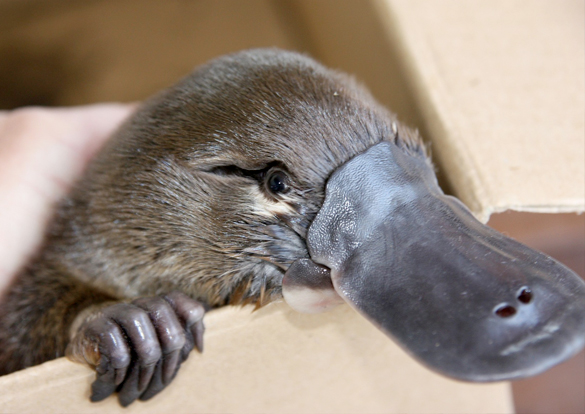
\includegraphics[width=\linewidth]{figures/platypusLg.jpg}
\end{frame}


\appendix
\bibliographystyle{alpha}
\bibliography{bibliography}
\nocite{*}

\end{document}
